\documentclass[11pt]{article}

\ifdefined\HGRUseCameraReady
  \usepackage[final]{vendor/acl}
\else
  \usepackage[review]{vendor/acl}
\fi

\usepackage{times}
\usepackage{latexsym}
\usepackage[T1]{fontenc}
\usepackage[utf8]{inputenc}
\usepackage{microtype}
\usepackage{inconsolata}
\usepackage{graphicx}
\usepackage{booktabs}
\usepackage{amsmath}
\usepackage{array}
\usepackage{xspace}

\newcommand{\hgrag}{HyperGranular-RAG\xspace}
\newcommand{\full}{\textsc{Full}\xspace}
\newcommand{\dense}{\textsc{Dense}\xspace}
\newcommand{\bge}{\textsc{BGE}\xspace}
\newcommand{\prot}{\textsc{Protected}\xspace}

\title{HyperGranular-RAG: Structured Evidence Completion\\
for Compact Multi-Hop Retrieval}

\def\HGRCameraReadyAuthorFile{camera_ready_author_block.tex}
% HyperGranular-RAG submission identity switch.
% Default: anonymous. Do not change the default in the tracked review source.
%
% Camera-ready use requires an explicit definition before this file is loaded:
%   \def\HGRUseCameraReady{1}
% It also requires a human-confirmed camera_ready_author_block.tex file.

\newif\ifhgrcameraready
\ifdefined\HGRUseCameraReady
  \hgrcamerareadytrue
\else
  \hgrcamerareadyfalse
\fi

\providecommand{\HGRAnonymousAuthorText}{Anonymous Authors}
\providecommand{\HGRCameraReadyAuthorFile}
  {paper/latex/camera_ready_author_block.tex}

\ifhgrcameraready
  \InputIfFileExists{\HGRCameraReadyAuthorFile}{}{%
    \PackageError{hypergranular-rag}{%
      Camera-ready identity file is missing%
    }{%
      Keep anonymous mode active, or create the identity file only after all
      author metadata has been confirmed by the human authors.%
    }%
  }
\else
  \author{\HGRAnonymousAuthorText}
\fi


\begin{document}
\maketitle

\begin{abstract}
Multi-hop retrieval-augmented generation must assemble complementary evidence
within a fixed context budget, yet relevance-only rankings may omit bridge
evidence and unconstrained expansion may displace useful items. We introduce
\hgrag, an inference-time evidence-completion framework that organizes
candidate sentences into adaptive granular balls, connects query-relevant
balls with facet hyperedges, and inserts a small number of candidates after a
protected dense prefix. Across three closed-candidate HotpotQA and MuSiQue
evaluations with Qwen2.5-1.5B-Instruct, \hgrag improves answer F1 over a
compact MiniLM retriever by $+0.01478$ [0.00020, 0.02988],
$+0.01140$ [0.00450, 0.01835], and $+0.01357$ [0.00491, 0.02233].
A matched ablation further shows a $+0.01336$ [0.00341, 0.02343] gain for
facet-conditioned selection over centroid-only expansion. With BGE
large-en-v1.5, the original system underperforms the strong dense baseline,
while cross-space and BGE-native extensions yield no statistically resolved
improvement. Holding the inserted set fixed, protected placement improves over
unprotected placement. These findings show that structured evidence completion
can recover evidence gaps for a compact retrieval backbone, while its marginal
value contracts with a stronger retriever. Paired bootstrap intervals,
pre-specified evaluation settings, and independent artifact verification
support these scoped conclusions.
\end{abstract}

\section{Introduction}

Retrieval-augmented generation (RAG) gives language models access to
non-parametric evidence at inference time
\citep{lewis2020rag,guu2020realm}. Dense passage retrieval provides an
effective learned relevance ordering \citep{karpukhin2020dpr}, but multi-hop
questions introduce a joint-coverage requirement: the selected context must
contain multiple pieces of evidence, not merely high-scoring passages
considered independently. HotpotQA and MuSiQue make this requirement explicit
through multi-hop questions and supporting-evidence annotations
\citep{yang2018hotpotqa,trivedi2022musique}.

Under a fixed Top-$k$ budget, recovering a missing bridge necessarily competes
with evidence already selected by the retriever. If individually similar units
occupy much of the ranking, a complementary bridge may remain outside the
generator context. Expansion can recover that bridge, but every insertion can
displace an item that the base retriever ranked highly.
Retrieved evidence is also not uniformly useful to a generator: position,
redundancy, prompt construction, and the generator itself affect whether a
retrieved item changes the answer \citep{liu2024lostmiddle,ram2023incontext}.
Evidence coverage, ranking placement, and answer utility must therefore be
measured separately.

\hgrag is a structured evidence-completion layer for dense retrieval under
this fixed context budget. It organizes sentence units into adaptive granular
balls, identifies cross-ball relations through query-aware facet hyperedges,
and inserts at most four eligible units after a protected Dense Top-10 prefix
while preserving an effective Top-20. After development-time configuration,
retrieval on confirmation data proceeds without access to answers,
supporting-fact labels, generator outputs, or downstream scores. Development
labels are used only for designated configuration selection and remain
separate from confirmation evaluation. Granular balls act as adaptive local
clusters in embedding space, while hyperedges represent higher-order relations
involving more than pairwise adjacency
\citep{xia2019granularball,feng2019hgnn}.

We evaluate whether structured evidence completion improves compact dense
retrieval and whether the same mechanism provides additional value with a
stronger retriever. The study covers pre-specified HotpotQA and MuSiQue
closed-candidate settings, matched component contrasts, one additional
generator configuration, a BGE large-en-v1.5 baseline, a cross-space BGE
sidecar, and a BGE-native reconstruction. Development choices remain separate
from confirmation, and independent verifiers reconstruct the reported
comparisons.

Our study yields three main findings. First, static \hgrag repeatedly improves
answer F1 over the compact MiniLM Dense backbone in the three Qwen evaluations.
Second, facet-conditioned selection improves over the specific centroid-only
NoFacet ablation within that system. Third, when the cross-space sidecar holds
the inserted candidate set constant, protected placement improves over direct
unprotected placement. The gains are backbone-dependent: the original system
falls below BGE, and neither tested BGE extension yields a statistically
resolved answer-quality improvement. Our conclusions are restricted to the
evaluated closed-candidate settings; open-domain retrieval, broader generator
transfer, and the independent necessity of granular balls remain open
questions.

We make three contributions:
\begin{itemize}
  \item We introduce a structured evidence-completion layer that combines
        adaptive granular-ball organization, query-aware facet hyperedges, and
        protected budget-constrained insertion under a fixed Top-$k$ budget.
  \item Through controlled HotpotQA and MuSiQue evaluations, we establish
        repeatable answer-F1 gains over a compact MiniLM retriever and matched
        evidence for facet-conditioned selection over centroid-only expansion.
  \item Through component, placement, generator-transfer, and strong-retriever
        studies, we characterize when structural completion provides marginal
        value and when that value contracts, with independently verifiable
        artifacts supporting the reported scope.
\end{itemize}

\section{Related Work}

\paragraph{Dense and multi-hop retrieval.}
Dense passage retrieval learns dual-encoder representations for efficient
passage ranking \citep{karpukhin2020dpr}. Multi-hop variants extend retrieval
from independent passages to evidence chains. Multi-Hop Dense Retrieval
conditions later retrieval on preceding evidence \citep{xiong2021mdr}, while
BeamDR uses beam search over dense reasoning paths \citep{zhao2021beamdr}.
PullNet iteratively expands from retrieved entities over text and knowledge
bases \citep{sun2019pullnet}, and IRCoT interleaves retrieval with
chain-of-thought reasoning \citep{trivedi2023ircot}. \hgrag is not an iterative
question-rewriting method. Within each fixed closed candidate set, it performs
a single bounded completion of an existing ranking.

\paragraph{Graph, hypergraph, and hierarchical retrieval.}
Structure-aware retrieval represents relations that a flat relevance ordering
can miss. RAPTOR retrieves from a tree of recursively summarized text
\citep{sarthi2024raptor}. HippoRAG combines a knowledge graph with personalized
propagation \citep{gutierrez2024hipporag}, and GNN-RAG uses graph-neural
retrieval over knowledge graphs \citep{mavromatis2025gnnrag}. GraphRAG targets
query-focused summarization using graph communities \citep{edge2024graphrag}.
\hgrag differs in its evidence unit, relation, and budget contract: adaptive
balls organize local sentence units; facets define query-conditioned
cross-ball hyperedges; and insertion preserves a dense prefix instead of
replacing the complete ranking. These graph systems address broader
construction and retrieval settings, whereas our study isolates bounded
completion within a fixed candidate set; direct comparison is left to future
work.

\paragraph{Evidence expansion and generation.}
Retrieval-enhanced models can expose external evidence, but the generator
still consumes a finite context. RECOMP studies selective and compressed
augmentation \citep{xu2024recomp}, while long-context studies show that
evidence position affects model use even when the information is present
\citep{liu2024lostmiddle}. Fusion-in-Decoder demonstrates the importance of
how multiple passages are consumed \citep{izacard2021fid}, and in-context RALM
shows that retrieved text can condition language models without parameter
updates \citep{ram2023incontext}. We therefore use paired answer F1 as the
primary endpoint and treat retrieval coverage as supporting evidence.

\paragraph{Alternative completion controls.}
A simpler completion rule could combine relevance with diversity or uncovered
query-term coverage without constructing higher-order relations. The NoFacet arm
in this study is narrower: it preserves granular-ball geometry and selects up
to two eligible balls by query-to-centroid score. It is therefore a matched
test of the pre-specified facet-conditioned selector against centroid-only ball
expansion, not a comparison with all relevance--diversity or coverage
objectives. We retain this distinction in every component claim.

\paragraph{Evaluation and negative evidence.}
KILT emphasizes provenance-aware evaluation in knowledge-intensive tasks
\citep{petroni2021kilt}. Reproducibility guidance motivates explicit
dependencies, artifacts, and reporting boundaries
\citep{pineau2021reproducibility}. Statistical uncertainty is not resolved by
relabelling an interval crossing zero as ``no effect'' or equivalence
\citep{amrhein2019retire}. We therefore report comparisons as supported,
negative, statistically unresolved, or without a matched estimand.

\section{HyperGranular-RAG}

\subsection{Problem Formulation}

For a query $q$, let $U_q=\{u_i\}$ be the closed candidate set of sentence
units. A fixed encoder maps the query and each
\texttt{title + ``. '' + sentence} unit to an L2-normalized representation. The base
relevance score is cosine similarity,
\begin{equation}
s(q,u_i)=\hat e_q^\top \hat e_i.
\end{equation}
Ties are resolved by ascending \texttt{unit\_id}. The Dense baseline returns
the first $K_q=\min(20,|U_q|)$ unique units. \hgrag constructs an additional
ordered set of eligible units but must return the same effective $K_q$. No
answer, gold supporting unit, or generator output enters this construction.

\subsection{Adaptive Granular Balls}

Each query's candidate embeddings begin as one root set. For a current ball
$B$, let
\begin{equation}
 c_B=\operatorname{norm}\left(\frac{1}{|B|}\sum_{i\in B}\hat e_i\right),\quad
 d_i=1-\hat e_i^\top c_B,
\end{equation}
with radius $r_B=\max_{i\in B}d_i$ and compactness
$1-|B|^{-1}\sum_{i\in B}d_i$. In the compact MiniLM variant, $B$ is split iff
its depth is below 6, $|B|\geq4$, and either $|B|>3$ or $r_B>0.78$. The first
seed is the unit farthest from $c_B$; the second has minimum cosine similarity
to the first. Each unit is assigned to the seed with higher cosine similarity.
A split is retained only when both children contain at least two units.
Ties preserve the candidate order. We keep these parameters fixed across
evaluation settings; they are not learned from confirmation data.

\subsection{Query-Aware Facet Hyperedges}

Each ball aggregates content terms from titles and sentences after fixed
ASCII-alphanumeric and stop-word rules. Its facet terms are the intersection
between ball terms and query terms. The two balls with highest query-to-centroid
cosine become seeds. A non-seed ball can form an expansion hyperedge only if it
introduces a new query term and passes fixed gates on ball size, ball score or
seed proximity, units per new term, and shared-term redundancy.
We use \emph{facet hyperedge} for this query-conditioned relation between the
seed balls and an expansion ball that contributes new query-term coverage.

For a candidate ball $B$, let $n_B$ be the number of query terms newly covered
beyond the seeds, $t_B$ the total number of query terms in $B$, $m$ the number
of query terms, $b_B=\hat e_q^\top c_B$, $a_B$ the maximum cosine to a seed
centroid, and $\rho_B$ the fraction of $B$'s facet terms already covered. The
compact-variant score is
\begin{equation}
\begin{split}
h_B={}&0.45\,n_B/\max(m,1)\\
     &+0.20\,t_B/\max(m,1)\\
     &+0.20\,b_B+0.15(1-a_B)\\
     &-0.20\rho_B-0.05|B|/8.
\end{split}
\end{equation}
A candidate must introduce at least one new term, contain at most 8 units,
satisfy $b_B\geq0.12$ or $a_B\geq0.05$, have at most 6 units per new term,
obey $\rho_B\leq0.90$, and have $h_B\geq0.10$. Candidates are ordered by
descending $h_B$ and then \texttt{edge\_id}; at most two distinct balls are
selected. Units inside an accepted ball remain ordered by original MiniLM
cosine and \texttt{unit\_id}; the fixed unit-level facet bonus is zero.
Consequently, the hyperedge selects candidate regions rather than learning a
new dense ranker.

\subsection{Protected Bounded Insertion}

The compact variant protects the first ten unique Dense units. \hgrag units
whose cosine is at least 0.1957079917192459 are considered in the pre-specified
order. At most four candidates absent from the protected prefix are
inserted immediately after that prefix. Remaining Dense units are appended in
their original order, followed only if necessary by unfilled expansion units,
and the result is truncated to $K_q$.

We set the candidate-score floor to 0.1957079917192459, the 25th percentile
selected during earlier development, and keep it fixed in all subsequent
evaluations (Table~\ref{tab:parameters}). We do not treat it as an independently
optimized value.

Protected insertion reduces the risk of displacing highly ranked evidence, but
it does not guarantee that an inserted candidate is useful. This distinction
motivates the placement and BGE comparisons below.

\subsection{Compact, Sidecar, and Native Variants}

The \emph{compact variant} uses MiniLM embeddings for the base ranking, ball
geometry, facet gates, and unit ordering. The \emph{cross-space sidecar} keeps
BGE Top-20 as the primary ranking while using the fixed MiniLM-\hgrag
structure to propose eligible candidates; no score fusion is introduced. The
\emph{BGE-native variant} reconstructs candidate geometry and structural
selection in BGE space under one configuration selected during development and
then fixed for confirmation. We evaluate the three variants separately because each isolates
a different interaction between structural completion and the base retriever.

With embeddings precomputed, the closed-candidate procedure is
$O(H|U_q|d+|U_q|\log|U_q|+|{\cal B}_q|\log|{\cal B}_q|)$; Appendix~A states
the component bounds and memory cost.

\begin{figure*}[t]
  \centering
  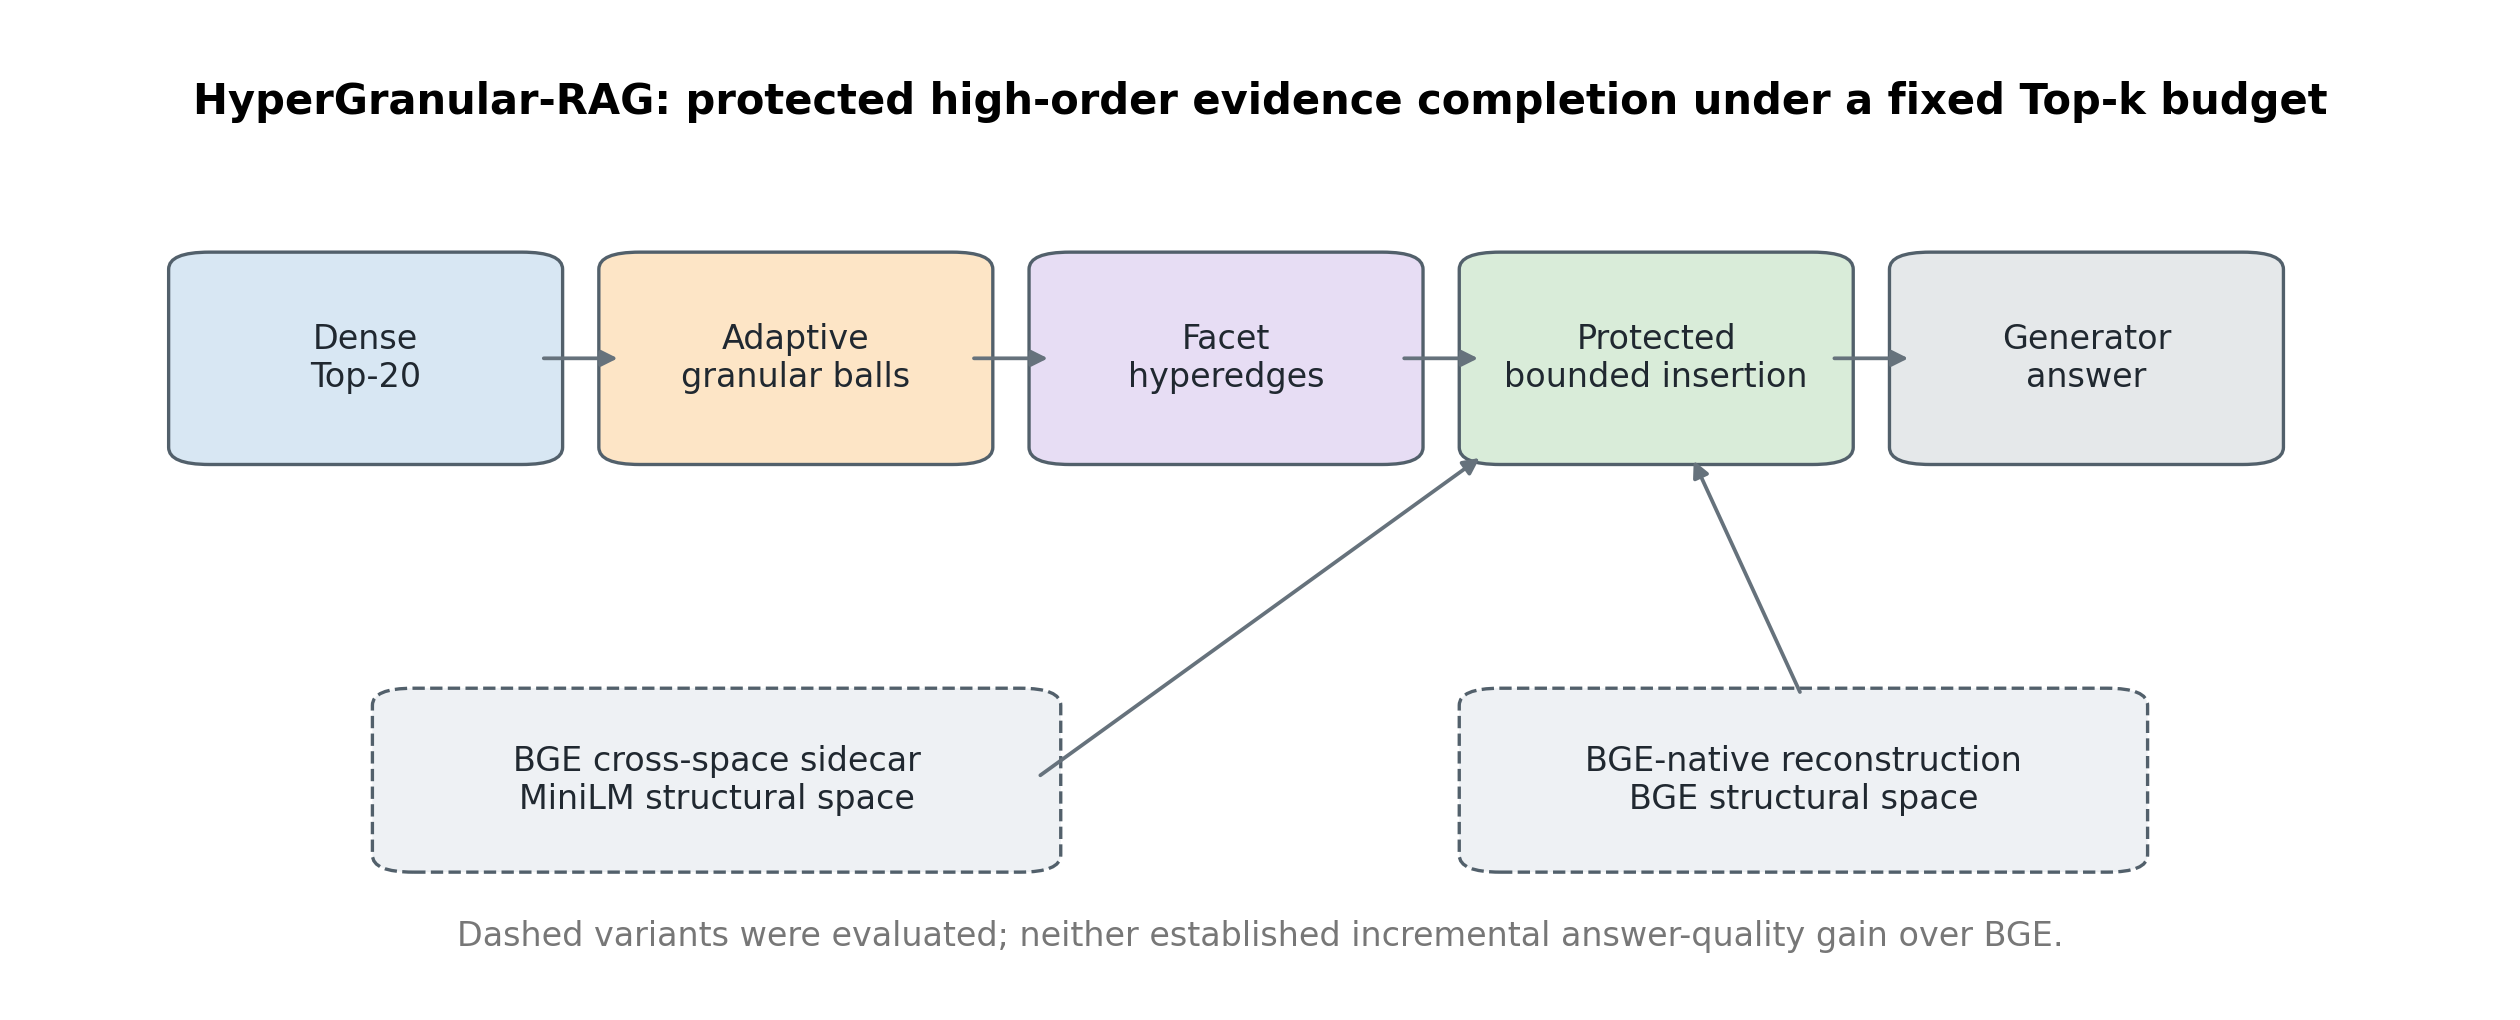
\includegraphics[
    width=\textwidth,
    trim=0 52bp 0 0,
    clip
  ]{../figures_stage5r/figure1_method_overview.png}
  \caption{\textbf{Overview of \hgrag and the evaluated retrieval variants.}
  Candidate units are ranked by a fixed dense retriever, organized into adaptive
  granular balls, connected through query-aware facet hyperedges, and inserted
  under a protected, bounded Top-$k$ policy before answer generation.
  Compact, cross-space sidecar, and BGE-native variants are evaluated
  separately rather than pooled. The right column distinguishes supported,
  negative, statistically unresolved, and unmatched outcomes, while the bottom row
  summarizes the scientific controls applied to the verified experiments.}
  \label{fig:method}
\end{figure*}

\section{Experiments}

\subsection{Datasets and Evaluation Settings}

HotpotQA provides diverse multi-hop questions and supporting facts
\citep{yang2018hotpotqa}; MuSiQue composes single-hop questions to reduce
shortcut solutions \citep{trivedi2022musique}. We evaluate retrieval within the
candidate sets supplied by each benchmark; corpus-scale indexing is outside the
scope of this study.

We evaluate the compact variant on 1,000 HotpotQA queries, 3,000 MuSiQue
queries, and a separate component set with 1,000 HotpotQA and 1,500 MuSiQue
queries. The cross-space sidecar and BGE-native confirmation studies each use a
separate, zero-overlap set with 1,000 HotpotQA and 1,500 MuSiQue queries. Query
selection is deterministic, and we verify dataset and query identities.

\subsection{Retrievers and Generators}

The compact baseline is the fixed MiniLM dense retriever used throughout the
original development program. BGE
large-en-v1.5 is the pre-specified strong dense baseline; the broader BGE
family is documented by \citet{xiao2023bge}, while the exact model revision is
bound in repository manifests.

The main generator is Qwen2.5-1.5B-Instruct FP16 with a fixed short-answer RAG
prompt and a 4,096-token input cap. One additional transfer evaluation uses
\texttt{google/gemma-4-E2B-it-qat-}\allowbreak
\texttt{mobile-transformers} in its official
mobile-QAT format. Because Qwen and Gemma use different numerical formats and
runtimes, this comparison characterizes the tested deployment configurations
rather than intrinsic architectural quality or cross-device efficiency.

\subsection{Experimental Design}

We specify all method and decision parameters before evaluating the
corresponding confirmation split. The BGE-native development study selected
configuration C10 with a development answer-F1 difference of $+0.003143$.
We use this development result only to select C10 and report its confirmation
performance separately. The pre-registered confirmation outcome ended the
BGE-native configuration search.

\subsection{Metrics and Statistical Decisions}

The primary endpoint is paired query-level answer-F1 difference. Answer exact
match (EM), retrieval complete recall at 20 (CR@20), and evidence recall at 20
(ER@20) are supporting endpoints. Each comparison uses 10,000 paired
bootstrap samples and pre-specified decision rules.
Dataset-joint comparisons assign equal weight to HotpotQA and MuSiQue. An
interval crossing zero is statistically unresolved and is not interpreted as
equivalence because no equivalence margin or formal equivalence test was
specified. Sample sizes define available resource and interval precision, not a
formal power guarantee.

\subsection{Label Access and Evaluation Integrity}

On confirmation data, candidate construction, retrieval, prompting, and
generation proceed without access to answer labels, supporting-fact
annotations, or evaluation feedback. Designated development labels may select
a configuration, including BGE-native C10, whereas confirmation labels remain
inaccessible until rankings, prompts, and predictions are fixed and are not
reused for selection. Thus ``label-free'' refers to retrieval execution rather
than the entire research process. Evaluators verify gold identity before
parsing it, and independent verifiers reconstruct ranking order, metrics,
bootstrap summaries, decisions, and artifact identities. Main/rerun identity
is checked in full or on a pre-hash deterministic subset.

\section{Results}

\begin{figure*}[t]
  \centering
  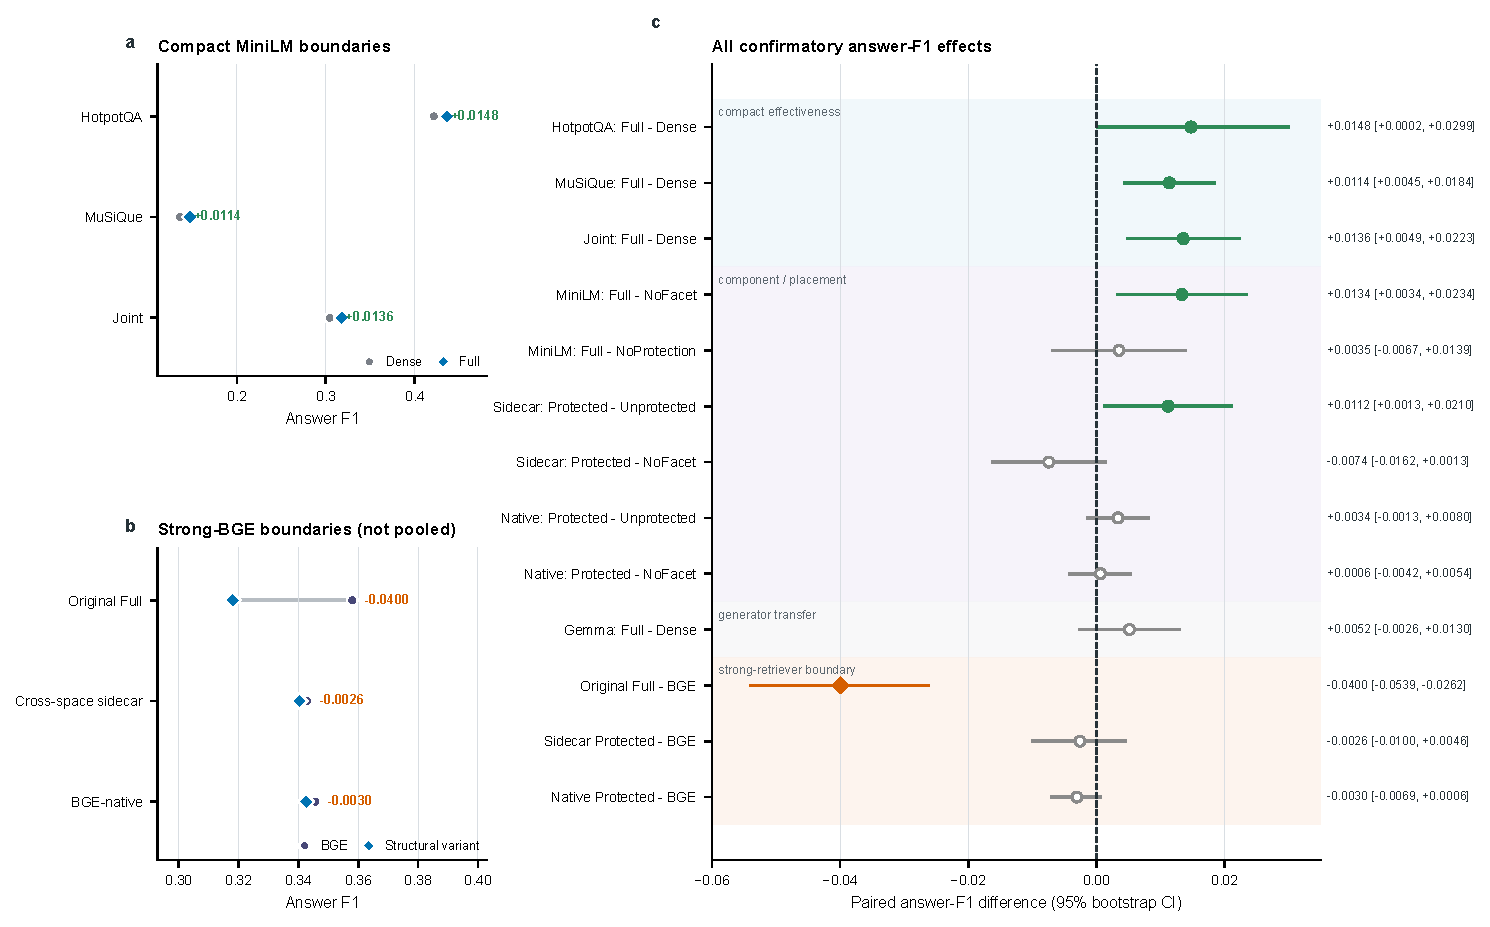
\includegraphics[width=\textwidth]{../figures_stage5r/figure2_main_performance_and_effects.pdf}
  \caption{\textbf{Main answer-F1 performance and paired effects.}
  Panels (a) and (b) compare absolute answer F1 only within matched frozen
  compact-MiniLM and strong-BGE boundaries; the three strong-BGE settings are
  not pooled. Panel (c) reports paired answer-F1 differences with
  pre-specified 95\% bootstrap confidence intervals. Hollow markers denote
  statistically unresolved comparisons, not equivalence.}
  \label{fig:main-effects}
\end{figure*}

\subsection{Repeated Gains over Compact Dense Retrieval}

Table~\ref{tab:compact} and Figure~\ref{fig:main-effects} show three Qwen
comparisons. On 1,000 HotpotQA queries, \full minus \dense answer F1 is
$+0.01478$ [0.00020, 0.02988]. On 3,000 MuSiQue queries, the difference is
$+0.01140$ [0.00450, 0.01835]. The separate joint component evaluation again
supports \full minus \dense with a dataset-equal-weight difference of
$+0.01357$ [0.00491, 0.02233].

\begin{table*}[t]
\centering
\scriptsize
\setlength{\tabcolsep}{2.5pt}
\begin{tabular}{@{}lccccccc@{}}
\toprule
Setting & F1 D/F & EM D/F & CR@20 D/F & ER@20 D/F &
Avg.\ ins. & F1 G/H & $\Delta$ F1 [95\% CI] \\
\midrule
HotpotQA & .42150/.43628 & .35600/.36600 & .73700/.79800 &
.87860/.90818 & 1.9300 & 47/34 & $+0.01478$ [.00020, .02988] \\
MuSiQue & .13595/.14735 & .10033/.11033 & .58900/.65000 &
.80553/.84128 & 2.4110 & 125/77 & $+0.01140$ [.00450, .01835] \\
Joint & .30446/.31803 & .25467/.26400 & .66617/.72217 &
.84529/.87657 & 2.1628 & 102/73 & $+0.01357$ [.00491, .02233] \\
\bottomrule
\end{tabular}
\caption{Absolute compact-dense outcomes and paired effects. D/F denotes
\dense/\full; G/H counts queries with positive/negative answer-F1 change.
Average insertions are structural candidates placed per query. The Joint row
is dataset-equal-weighted for absolute metrics; G/H and insertions use all
2,500 queries. All G/H and insertion counts are descriptive reconstructions
from fixed rankings and query records.}
\label{tab:compact}
\end{table*}

\hgrag improves answer F1 in all three compact-retriever evaluations, with
effect sizes from $+0.01140$ to $+0.01478$. These gains apply to the MiniLM
backbone, Qwen generator, fixed prompt, closed candidates, and Top-20 budget;
the strong-retriever experiments below evaluate whether the pattern extends to
BGE.

\subsection{Component Evidence}

Within the fixed MiniLM system, \full minus NoFacet is
$+0.01336$ [0.00341, 0.02343], supporting an incremental role for facet
conditioning relative to the specific centroid-only ball selector. This
matched contrast isolates facet conditioning within the granular-ball
candidate pool; generic relevance--diversity and coverage selectors remain
outside the present comparison. \full minus NoProtection is $+0.00354$
[$-0.00675$, 0.01389], so the independent contribution of protection is
statistically unresolved in that setting. We do not report a flat-unit
granular-ball ablation because ball seeds, split gates, edge budgets, and radii
have no unique matched counterparts at the unit level. This missing matched
estimand provides no evidence for or against a granular-ball effect.

In the cross-space sidecar, the inserted set is identical between protected
and unprotected conditions. \prot minus Unprotected is
$+0.01122$ [0.00129, 0.02104], which supports the placement rule within that
specific sidecar. However, \prot minus NoFacet is
$-0.00743$ [$-0.01616$, 0.00132], statistically unresolved. In BGE-native space,
\prot minus Unprotected is $+0.003367$ [$-0.001285$, 0.008026], and
\prot minus NoFacet is $+0.000631$ [$-0.004220$, 0.005365]; both are
statistically unresolved. Component effects are therefore system-dependent.

\begin{table}[t]
\centering
\scriptsize
\setlength{\tabcolsep}{2.2pt}
\begin{tabular}{@{}lll@{}}
\toprule
Contrast & $\Delta$ F1 [95\% CI] & State \\
\midrule
MiniLM facet & $+0.01336$ [0.00341, 0.02343] & Supported \\
MiniLM protection & $+0.00354$ [$-0.00675$, 0.01389] & Unresolved \\
Sidecar placement & $+0.01122$ [0.00129, 0.02104] & Supported \\
Sidecar facet & $-0.00743$ [$-0.01616$, 0.00132] & Unresolved \\
Native placement & $+0.00337$ [$-0.00129$, 0.00803] & Unresolved \\
Native facet & $+0.00063$ [$-0.00422$, 0.00536] & Unresolved \\
Flat-ball control & --- & Not defined \\
\bottomrule
\end{tabular}
\caption{Complete component evidence. ``Native'' denotes the BGE-native
confirmation setting; effects are not transported between semantic spaces.
The flat-ball row has no matched estimand.}
\label{tab:components}
\end{table}

\subsection{Comparison with a Strong Dense Retriever}

The pre-specified BGE baseline outperforms original \full. The
dataset-equal-weight \full minus BGE difference is
$-0.03998$ [$-0.05393$, $-0.02621$]. The complete interval lies below zero,
distinguishing this negative result from a statistically unresolved contrast.
On this evaluation, the original MiniLM-based \hgrag system performs below the
BGE baseline.

On the same joint component setting, BM25 and a Dense--BM25 hybrid provide
additional reference points.
\full minus BM25 is $-0.00755$ [$-0.02259$, 0.00773], and \full minus a
Dense--BM25 hybrid is $-0.00320$ [$-0.01591$, 0.00942]. Both comparisons are
statistically unresolved. BGE is the stronger reference point because the
entire \full-minus-BGE interval is negative.

\subsection{Cross-Space Sidecar Evaluation}

The cross-space sidecar asks whether the fixed MiniLM structural expansion can
add complementary candidates while BGE retains the primary ranking. Its core
\prot minus BGE difference is $-0.00256$ [$-0.00998$, 0.00458].
The sidecar comparison therefore remains statistically unresolved relative to
BGE. The positive protected-placement contrast answers a different question:
better placement of a fixed inserted set does not show that the set itself
improves BGE.

\subsection{BGE-Native Reconstruction}

The BGE-native study removes the cross-space mismatch by rebuilding candidate
geometry and facets in BGE space. Its confirmation comparison remains
statistically unresolved. The
dataset-equal-weight \prot minus BGE answer-F1 difference is
$-0.003046$ [$-0.006880$, 0.000631]; the EM difference is
$-0.003667$ [$-0.007667$, 0.000004]. Dataset-specific F1 differences are
$-0.002907$ [$-0.008682$, 0.002652] for HotpotQA and
$-0.003184$ [$-0.008486$, 0.001863] for MuSiQue. Both point estimates are
slightly negative, but all intervals cross zero. The tested BGE-native
reconstruction therefore provides no statistically resolved answer-quality
improvement over BGE in this setting.

\begin{table}[t]
\centering
\scriptsize
\setlength{\tabcolsep}{2.2pt}
\begin{tabular}{@{}lll@{}}
\toprule
Setting & $\Delta$ F1 [95\% CI] & State \\
\midrule
Gemma transfer & $+0.00516$ [$-0.00262$, 0.01295] & Unresolved \\
Full vs.\ BM25 & $-0.00755$ [$-0.02259$, 0.00773] & Unresolved \\
Full vs.\ hybrid & $-0.00320$ [$-0.01591$, 0.00942] & Unresolved \\
Full vs.\ BGE & $-0.03998$ [$-0.05393$, $-0.02621$] & Negative \\
Sidecar vs.\ BGE & $-0.00256$ [$-0.00998$, 0.00458] & Unresolved \\
Native vs.\ BGE & $-0.00305$ [$-0.00688$, 0.00063] & Unresolved \\
\bottomrule
\end{tabular}
\caption{Strong-retriever comparisons and generator transfer. Each row uses
its own evaluation setting; rows are not pooled.}
\label{tab:strong}
\end{table}

The positive C10 development difference is not pooled with this result:
development selected the configuration, and the separate confirmation split
evaluated it.

\subsection{Generator Transfer}

Under the single pre-specified Gemma mobile-QAT configuration, the
dataset-equal-weight \full minus \dense difference is
$+0.00516$ [$-0.00262$, 0.01295], which is statistically unresolved. This
transfer result applies only to the tested Qwen FP16 and Gemma mobile-QAT
deployment configurations on the recorded RTX 4060 Laptop 8GB, fixed
short-answer prompt, and 4,096-token cap.

\subsection{Efficiency and Evidence Displacement}

These measurements describe the recorded hardware rather than cross-device
efficiency. For the BGE-native confirmation run, retrieval
reconstruction took 8.544 seconds; BGE and BGE-native \prot generation took
887.650 and
884.198 seconds, respectively; recorded GPU peak memory was 3.592 GiB.

Post hoc supporting-evidence analysis clarifies why coverage and answer quality diverge
(Figure~\ref{fig:coverage-utility}). In the BGE-native \prot condition,
HotpotQA adds 3 gold units, displaces 2, and has net $+1$; MuSiQue adds 16,
displaces 15, and also has net $+1$. Nevertheless, answer-F1 point estimates
relative to BGE are negative. In the cross-space sidecar, HotpotQA has 21
added, 29 displaced, and net $-8$, whereas MuSiQue has 59 added, 50 displaced,
and net $+9$. These counts are post-decision descriptive analyses and were not
used to retune the method.

\section{Discussion}

\paragraph{Why compact retrieval can benefit.}
The repeated MiniLM gains support a focused interpretation: when a
compact representation leaves recoverable evidence gaps, local candidate
organization plus query-conditioned cross-ball expansion can expose
complementary units that a flat ranking omits. The joint component
confirmation's facet contrast supports facet-mediated candidate selection
within that implementation. The Gold-free mechanism summaries in
Figure~\ref{fig:mechanism} show that insertions remain bounded and that
eligible sidecar candidates often lie beyond BGE's Top-20; these descriptive
patterns do not establish causal mediation. We therefore interpret the repeated gains as
evidence that structured completion can recover complementary units omitted by
this compact retriever.

\paragraph{Why the increment contracts under strong BGE.}
BGE begins with substantially higher answer quality than the original MiniLM
system. The original \full ranking is clearly worse than BGE, and both tested
extensions around BGE yield narrow intervals around small negative point
estimates. A stronger representation may already rank much of the recoverable
evidence highly, leaving less marginal opportunity for structural expansion.
Additional units then compete with already strong evidence. These results show
that the marginal value of the tested structural completion contracts with
BGE; they do not determine whether other structure-aware approaches can
complement strong retrievers.

\paragraph{Evidence addition is not evidence utility.}
The BGE-native confirmation is especially informative: net gold evidence
increases slightly, but answer quality does not. A gold-labelled unit can be redundant
with retained context,
weakly positioned, difficult for the generator to use, or offset by a
different displacement. Conversely, a non-gold unit can affect the answer.
CR/ER, gold transitions, and answer F1 therefore answer different questions.
The fixed representative cases in Figure~\ref{fig:qualitative} illustrate both
an inserted supporting unit that repairs an answer and a displacement that
removes supporting evidence; the examples are descriptive rather than
confirmatory.

\paragraph{Placement matters but cannot substitute for efficacy.}
The cross-space sidecar placement result isolates ranking position because
protected and unprotected conditions contain the same inserted set. It
supports preserving high-ranked evidence under a fixed budget. However, the
BGE-native confirmation does not independently confirm the placement
increment, and neither placement
experiment establishes that \prot exceeds BGE.

\paragraph{Facet effects depend on semantic space.}
Facet-conditioned selection beats the centroid-only NoFacet arm in the fixed
MiniLM system, but its increments are statistically unresolved in cross-space and
BGE-native studies. Query-to-ball geometry, seed identities, facet eligibility,
and competition with the base ranking all depend on representation space. The
MiniLM effect is therefore neither transported to BGE nor interpreted as
superiority over untested diversity/coverage selectors.

\paragraph{Selection and displacement explain failure modes.}
Post-label controller analyses locate failure at selection and displacement:
resource budgeting retained harm more often than gain, the query-level score
reversed direction, and a candidate-level probe remained below its advancement
gate (Table~\ref{tab:failure-audit}). These development results are
explanatory, not confirmation; complementary-candidate detection remains open.

\paragraph{Separating development from confirmation.}
The positive BGE-native development result motivated one pre-specified
confirmation evaluation. It did not license retroactive configuration search
after confirmation. We therefore report the confirmation result without
further tuning on the confirmation set.

\paragraph{Interpreting statistically unresolved comparisons.}
The sidecar, BGE-native, and generator-transfer intervals cross zero. Without a
pre-specified equivalence margin and an equivalence test, these results cannot
be called equal. They also do not establish harm.

\section{Limitations}

Evaluation is closed-candidate rather than full-wiki or open-domain; it does
not measure indexing, approximate-nearest-neighbor recall, or corpus-scale
noise. The repeated positive evidence uses one Qwen generator, and the only
additional generator is a single Gemma mobile-QAT configuration. Only one
strong BGE backbone is tested. The BGE-native configuration family is finite
and development-selected; untested variants remain unknown.

A scientifically matched flat granular-ball control was not defined, so the
granular-ball structure lacks an independent ablation claim. Protected
insertion has inconsistent independent evidence: cross-space sidecar placement
is supported, while the joint-component and BGE-native protection-related
contrasts are statistically unresolved. Facet evidence is representation- and
implementation-dependent.
No matched relevance--diversity, maximum-coverage, or other simple completion
selector was evaluated, so the hyperedge representation has not been shown
necessary or superior to such alternatives.

The HotpotQA training split may have appeared in generator pretraining. The
project can guarantee only that its own retrieval and evaluation respected the
pre-specified data separation. Post hoc mechanism analyses are descriptive, not
confirmatory causal analyses. Sample sizes reflect available resources and
interval precision, not a formal power design. No statistically unresolved result is
evidence of equivalence.

\section{Reproducibility}

The repository records exact dataset and model revisions, configurations,
rankings, predictions, and evaluation outputs. Independent scripts reconstruct
the reported metrics and decisions from these artifacts. Every plot has a
machine-readable source, and the manuscript build is deterministic. Licenses
are recorded separately; caches and third-party weights are excluded.

\section{Conclusion}

\hgrag provides repeatable answer-F1 gains for the compact MiniLM retriever
across three closed-candidate evaluations, and facet-conditioned selection
improves over its centroid-only comparator. The BGE experiments show that this
increment is backbone-dependent: the original MiniLM-based system performs
below BGE, while the cross-space and BGE-native extensions remain statistically
unresolved. Protected placement can improve the ordering of a fixed candidate
set, but candidate selection remains central to end-to-end answer quality.
Overall, structured evidence completion is useful in the evaluated compact
retrieval setting, while its value with stronger retrievers remains an open
methodological problem.

\section*{Ethical Considerations}

This study uses existing benchmark datasets and publicly documented model
artifacts. It does not recruit human participants or collect new personal data.
The analysis reports negative, statistically unresolved, and unmatched results
alongside positive findings to reduce selective-reporting risk. A venue-specific
determination of whether a formal institutional ethics statement is required
remains subject to human confirmation.

\section*{Data and Code Availability}

The identity-exposing development repository records code, configurations,
frozen derived evaluation artifacts, figure source data, and verification
manifests. It is not linked in this anonymous draft. Original benchmark
datasets, model weights, and large local caches are not redistributed and must
be obtained from their official sources under their respective terms. An
anonymous artifact snapshot and final reuse license remain pending human
decisions.

\section*{Generative AI Disclosure (Draft)}

Generative AI tools were used for code assistance, experiment-workflow
assistance, documentation assistance, and language-editing assistance. They
are not authors and do not bear academic responsibility. Human authors retain
responsibility for the scientific design, evidence selection, verification,
claims, and submitted text. Final wording will be reviewed against the selected
venue's policy before submission.

\bibliography{../references/verified_references}

\appendix

\section{Deterministic Procedures and Fixed Parameters}

\paragraph{Algorithm 1: adaptive granular-ball construction.}
Initialize a queue with $(U_q,0)$. For each ball $B$ at depth $z$, compute
$c_B$ and $r_B$. If the depth, size, and radius/size gates do not permit a
split, emit $B$. Otherwise choose the first seed as the unit farthest from
$c_B$, choose the second as the unit least similar to the first, and assign
each unit to its more similar seed. Candidate-order ties go to the earlier
seed. Accept the split only if both children have at least two units; otherwise
emit $B$. Continue until the queue is empty. Stable candidate order and
\texttt{unit\_id} resolve remaining ties.

\paragraph{Algorithm 2: query-aware facet-hyperedge selection.}
Tokenize the query and every ball with the frozen rules, intersect each ball's
term set with the query-term set, and select the two highest
query-to-centroid balls as seeds. Compute newly covered terms and the frozen
$h_B$ score for every non-seed ball. Reject balls that fail any eligibility
gate. Sort survivors by $( -h_B,\texttt{edge\_id})$, retain at most two
distinct balls, and order their units by original MiniLM cosine and
\texttt{unit\_id}. No Gold label or answer score enters this procedure.

\paragraph{Algorithm 3: protected bounded insertion.}
Let $K_q=\min(20,|U_q|)$ and protect the first $\min(10,K_q)$ unique Dense
units. Traverse the eligible expansion order, retain units at or above the
frozen score floor, skip protected duplicates, and place at most four units
immediately after the prefix. Append unused Dense units in their original
order, then expansion units only if needed to fill $K_q$. Deduplicate stably
and truncate to $K_q$.

\paragraph{Complexity.}
For $n=|U_q|$, $B=|{\cal B}_q|$, embedding dimension $d$, and maximum depth
$H$, Dense scoring/sorting costs $O(nd+n\log n)$; recursive two-seed
assignment costs $O(Hnd)$; facet scoring and ordering costs
$O(n+Bd+B\log B)$ apart from tokenization; insertion costs $O(n)$. Working
memory is $O(nd+n+B)$. Encoder and generator inference are excluded.

\begin{table*}[h]
\centering
\scriptsize
\setlength{\tabcolsep}{3pt}
\begin{tabular}{@{}p{0.24\textwidth}p{0.31\textwidth}p{0.39\textwidth}@{}}
\toprule
Group & Fixed value & Provenance and sensitivity status \\
\midrule
Ball split & depth $<6$; splittable size $\geq4$; radius gate 0.78;
minimum child size 2 & Frozen compact implementation; no confirmatory
sensitivity sweep \\
Ball seeds and ties & farthest from centroid; then least similar to seed 1;
stable candidate order & Deterministic rule, not learned \\
Facet seeds/budget & 2 seed balls; at most 2 expansion balls & Frozen compact
implementation; no confirmatory budget sweep \\
Facet gates & new terms $\geq1$; ball size $\leq8$; $b_B\geq.12$ or
$a_B\geq.05$; units/new term $\leq6$; redundancy $\leq.90$; $h_B\geq.10$ &
Frozen compact implementation \\
Facet score weights & $.45,.20,.20,.15,-.20,-.05$; unit bonus 0 & Frozen
implementation weights; no claim of global optimality \\
Insertion & protected prefix 10; budget 4; effective $K=20$ & Frozen
transferred policy \\
Candidate floor & 0.1957079917192459 & Stage2E calibration 25th percentile,
transferred exactly; not an independently established optimum \\
Ordering & descending cosine or $h_B$, then \texttt{unit\_id} or
\texttt{edge\_id} & Fully deterministic tie-breaking \\
\bottomrule
\end{tabular}
\caption{Fixed compact-method parameters. ``No confirmatory sensitivity
sweep'' is a limitation, not evidence of robustness. BGE-native development
used a separate finite configuration family and is not pooled with this table.}
\label{tab:parameters}
\end{table*}

\paragraph{Additional frozen results and analyses.}
The following tables and figures report absolute strong-retriever outcomes,
coverage--utility relationships, Gold-free retrieval behavior, representative
cases, efficiency, and the supported-claim boundary. Confirmatory and
post-decision descriptive evidence remain explicitly separated.

\begin{table*}[h]
\centering
\small
\setlength{\tabcolsep}{5pt}
\begin{tabular}{@{}llcccc@{}}
\toprule
Evaluation setting & Method & F1 & EM & CR@20 & ER@20 \\
\midrule
Joint component (Stage4H) & BGE & .35801 & .30467 & .85400 & .93902 \\
Joint component (Stage4H) & Original \full & .31803 & .26400 & .72217 & .87657 \\
Cross-space sidecar (Stage4I) & BGE & .34301 & .28000 & .84967 & .93594 \\
Cross-space sidecar (Stage4I) & \prot & .34045 & .27767 & .84350 & .93459 \\
BGE-native confirmation (Stage5A) & BGE & .34569 & .28500 & .86167 & .94288 \\
BGE-native confirmation (Stage5A) & \prot & .34264 & .28133 & .86233 & .94288 \\
\bottomrule
\end{tabular}
\caption{Dataset-equal-weight absolute outcomes in the strong-retriever
evaluations. Comparisons are valid only within the same setting; rows from
different settings are not pooled.}
\label{tab:absolute-strong}
\end{table*}

\begin{figure*}[t]
  \centering
  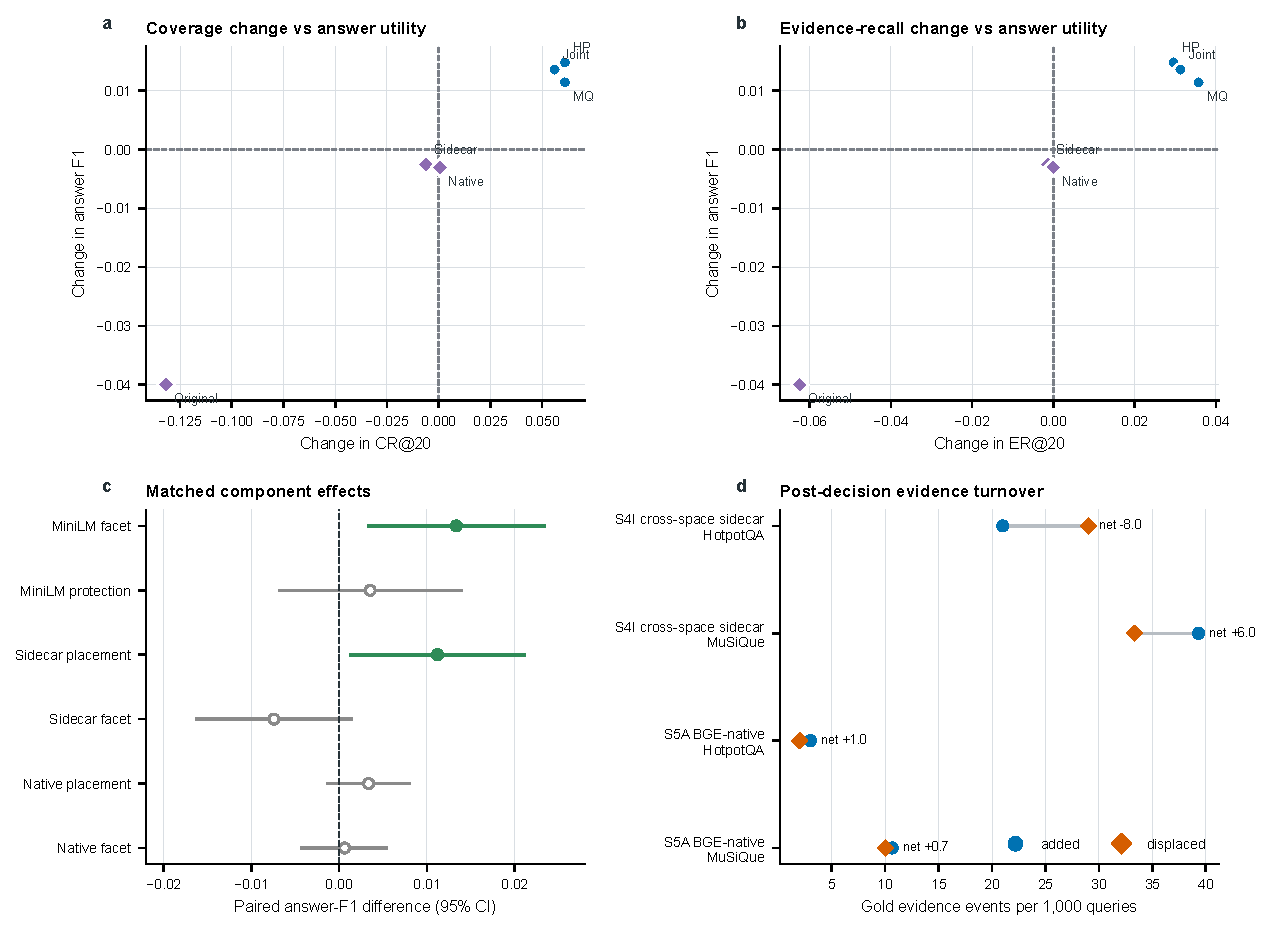
\includegraphics[width=\textwidth]{../figures_stage5r/figure3_coverage_utility_and_ablation.pdf}
  \caption{\textbf{Coverage, answer utility, component effects, and evidence
  turnover.} Panels (a) and (b) plot within-boundary changes in CR@20 and ER@20
  against answer F1, keeping compact and strong-retriever settings visually
  distinct. Panel (c) reports matched component effects with 95\% bootstrap
  confidence intervals. Panel (d) reports post-decision descriptive Gold
  evidence events per 1,000 queries. Coverage or evidence addition alone does
  not imply answer improvement.}
  \label{fig:coverage-utility}
\end{figure*}

\begin{figure*}[t]
  \centering
  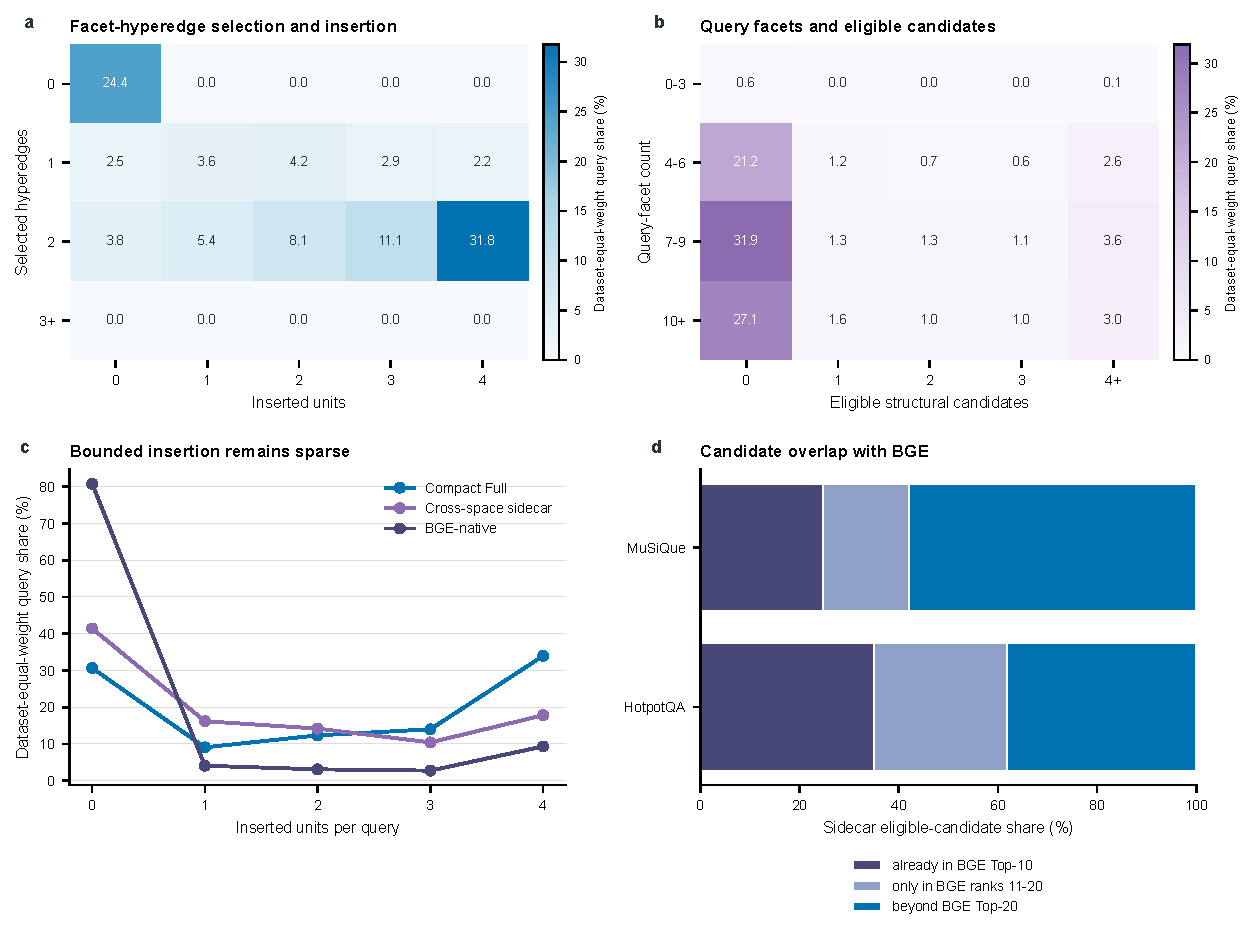
\includegraphics[width=\textwidth]{../figures_stage5r/figure4_mechanism_analysis.pdf}
  \caption{\textbf{Descriptive retrieval mechanism analysis.}
  Panel (a) relates selected facet hyperedges to bounded insertions in the
  compact joint evaluation. Panel (b) relates query-facet counts to eligible
  BGE-native candidates. Panel (c) reports insertion-count distributions
  separately for compact, cross-space sidecar, and BGE-native settings.
  Panel (d) decomposes sidecar-eligible candidates by overlap with the BGE
  Top-20. All panels are Gold-free descriptive reconstructions and do not
  establish causal mediation.}
  \label{fig:mechanism}
\end{figure*}

\begin{figure*}[t]
  \centering
  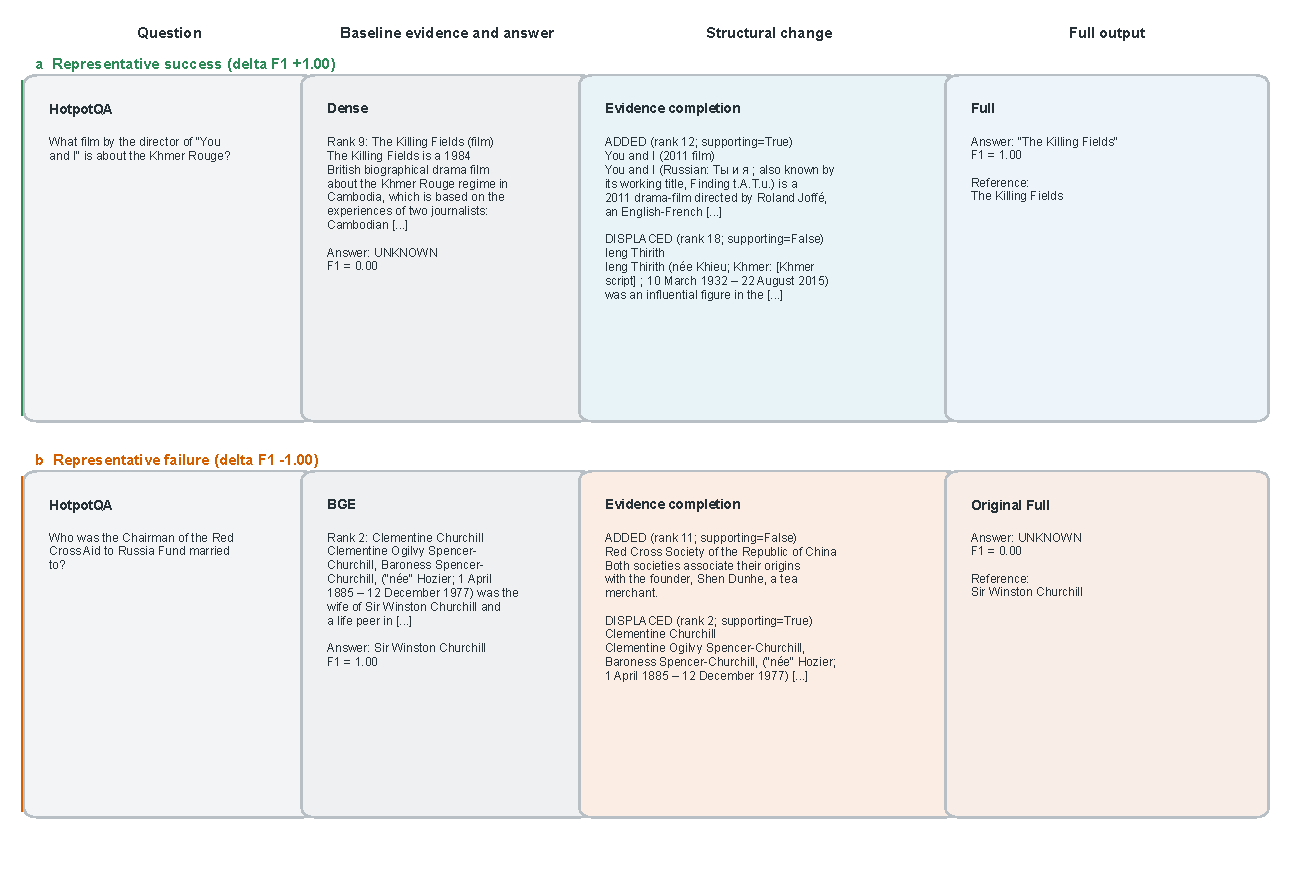
\includegraphics[width=\textwidth]{../figures_stage5r/figure5_qualitative_cases.pdf}
  \caption{\textbf{Fixed representative success and failure cases.}
  The success case is the deterministic median representative among events
  with positive Full-minus-Dense answer-F1 change, increased CR@20, and an
  inserted supporting unit. The failure case is selected analogously among
  events with negative Original-Full-minus-BGE answer-F1 change and a
  displaced supporting unit. Both are post-decision descriptive examples.
  The source CSV preserves frozen text verbatim; a Khmer-script span is
  abbreviated in the rendered panel for publication-font compatibility.}
  \label{fig:qualitative}
\end{figure*}

\begin{table*}[h]
\centering
\small
\begin{tabular}{@{}p{0.23\textwidth}p{0.49\textwidth}p{0.22\textwidth}@{}}
\toprule
Layer & Observation & Evidential role \\
\midrule
Static expansion & Repeated compact-MiniLM answer-F1 gains, but query-level
gain and harm coexist & Confirmatory, bounded \\
Resource controller & Retained 47/94 gain and 53/69 harm queries; retention
gap $-0.26812$; two of six gates passed & Valid negative development result \\
Query score & Gain-vs-harm AUROC 0.39269 [0.30558, 0.48150] & Exploratory,
direction reversed \\
Candidate probe & AUROC 0.64310 [0.55520, 0.72974], AP 0.72198; Brier 0.26321
vs.\ 0.25338 prevalence baseline & Exploratory, unresolved \\
Strong-retriever displacement & Small or mixed net Gold changes did not yield
positive answer-F1 relative to BGE & Post-decision descriptive \\
\bottomrule
\end{tabular}
\caption{Failure analysis from Stage4B--Stage4D and the strong-retriever
evaluations. Exploratory and post-decision rows explain observed failure modes but
do not create new confirmatory claims.}
\label{tab:failure-audit}
\end{table*}

\begin{table*}[h]
\centering
\small
\begin{tabular}{@{}lll@{}}
\toprule
Item & Value & Evidential role \\
\midrule
Stage5A retrieval reconstruction & 8.544 s & Hardware-bound descriptive \\
Stage5A BGE generation & 887.650 s & Hardware-bound descriptive \\
Stage5A native Protected generation & 884.198 s & Hardware-bound descriptive \\
Stage5A GPU peak memory & 3.592 GiB & Hardware-bound descriptive \\
Bootstrap & 10,000 iterations per frozen decision & Confirmatory \\
Gold policy & Isolated until rankings/predictions were frozen & Integrity \\
Verification & Independent final verifiers passed & Integrity \\
\bottomrule
\end{tabular}
\caption{Efficiency and verification summary. Time and memory values do not
support cross-device efficiency claims.}
\label{tab:efficiency}
\end{table*}

\begin{table*}[h]
\centering
\small
\begin{tabular}{@{}p{0.39\textwidth}p{0.16\textwidth}p{0.37\textwidth}@{}}
\toprule
Claim & Evidence state & Setting \\
\midrule
Compact \full exceeds \dense in three evaluation settings & Supported &
MiniLM, Qwen, closed-candidate Top-20 \\
Facet increment in the fixed MiniLM system & Supported & Stage4H only \\
Protected placement with identical sidecar insertions & Supported &
Stage4I only \\
Original \full exceeds strong BGE & Negative & Stage4H \\
Cross-space sidecar exceeds BGE & Unresolved & Stage4I \\
BGE-native \prot exceeds BGE & Unresolved & Stage5A \\
BGE-native placement increment & Unresolved & Stage5A \\
BGE-native facet increment & Unresolved & Stage5A \\
Additional-generator transfer & Unresolved & One Gemma mobile-QAT setting \\
Flat granular-ball control & Unmatched & No matched estimand \\
Granular balls are necessary & Not established & Flat contrast undefined \\
Facet hyperedges beat generic diversity/coverage & Not tested & No matched
alternative selector \\
Open-domain deployment value & Not tested & Closed candidates only \\
\bottomrule
\end{tabular}
\caption{Scope of the manuscript's supported conclusions. Statistically
unresolved rows are not equivalence claims, and system-specific component
evidence is not transported across representation spaces.}
\label{tab:claims}
\end{table*}

\end{document}
